\chapter{The CMS experiment at the LHC}
\label{ch:LHC-CMS}

The whole work presented in this thesis is based on data collected by the
Compact Muon Solenoid (CMS) experiment~\cite{Chatrchyan:2008aa}, one of the four main experiments
installed along the Large Hadron collider (LHC) circumference~\cite{Evans:2006tq}. In this chapter,
a description of the entire experimental apparatus is provided: after an overview
on the LHC collider, the main CMS subdetectors used for particle 
identification and reconstruction are presented. 

%%%%%%%%%%%%%%%%%%%%%%%%%%%%%%%%%%%%%%%%%%%%%%%%%%%
\section{The Large Hadron Collider}
\label{sec:LHC}
%%%%%%%%%%%%%%%%%%%%%%%%%%%%%%%%%%%%%%%%%%%%%%%%%%%

The LHC technical features have to be framed thinking about the motivation behind the
building of this machine, the world's largest and powerful accelerator of protons. 
The unique experimental conditions achieved follows the need of addressing all 
the fundamental questions which LHC has been built for: 
proving the existence of the SM Higgs boson, discovering extended symmetries
or extra dimentions requires energy of tens of \tev and a huge number of collisions.

% it would be impossible achieving
%the same physics goals LHC aims to, accelerating electrons (and positrons), because of the loss
%of energy by synchrotron radiation. Also proton-antiproton collisions, used at Tevatron, 
	%do not match the need of achieving the luminosity requested, due to the limited production efficiency
%and collimation of antiprotons and also to the different internal nucleons structure. 

The LHC is hosted inside the former LEP 27~\si{km}-long tunnel, located under both French and Swiss
territory. The collider is carachterized by 16 superconducting radio-frequency (RF) accelerating cavities, 
focusing quadrupole magnets and 1232 superconducting dipole magnets for bending the protons 
and operating with a magnetic field of 8.3~\si{T}. In order to maintain superconductive properties, 
magnetic coils and superconductors are cooled at 1.9~$^\circ$\si{K} with superfluid Helium. 
Two beam pipes host protons circulating in opposite direction.
In order to be accelerated by RF cavities, proton beams have to be bunched: 
the LHC has been designed to contain 2808 bunches of $10^{11}$ protons each, 
with a separation in time of 25~\ns. The istantaneous luminosity, which is the number 
of particles per unit area per unit time and is indicated as $\mathcal{L}(t)$, 
is given by~\cite{Bayatian:2006zz}

%##########################################################################################################
\begin{equation}
    \mathcal{L}(t)=\frac{\gamma f k_B N^2_p}{4\pi \epsilon_n \beta^*} F
    \label{eq:INSTAlumi}
\end{equation} 
%##########################################################################################################

where $\gamma=E_{beam}/m_p$ is the Lorentz factor of protons in the beam, 
$f$ is the bunch frequency, $k_B$ is the number of bunch per beam, 
$N_p$ is the number of protons per bunch, $F$ is a reduction factor due
to a non-$\pi$ intersecting angle of the beams. $\epsilon_n$, the transverse emittance, and
$\beta^*$, the betatron function, both quantify the beam focusing by the magnetic optics
at the interaction point. Using the designed parameters and assuming $E_{beam}=$7~\tev,
the instantaneous luminosity reached is $\mathcal{L}=$10$^{34}$\cm$^{-2}$\si{s}$^{-1}$.
The averaged number of events for a given process with cross-section $\sigma$ (\si{cm}$^2$) is given by 

%##########################################################################################################
\begin{equation}
    N=\int \sigma \mathcal{L}(t) dt\mbox{ .}
    \label{eq:rate}
\end{equation} 
%##########################################################################################################

Four different experiments are located along the accelerator ring,
corresponding to the collision points of the two proton beams: ATLAS (``A Toroidal LHC Apparatus'')~\cite{Aad:2008zzm},
CMS~\cite{Chatrchyan:2008aa}, LHCb~\cite{Alves:2008zz} and ALICE (``A Large Ion Collider Experiment'')~\cite{Aamodt:2008zz}.
ATLAS and CMS are general-purpouse experiments and they are devoted to investigate a wide range of physics,
LHCb is designed to study $b$-physics and the CP-violation, ALICE is specilized in 
studying heavy ions and the quark-gluon pasma.

The LHC started its operation on September 2008, to be stopped 9 days later
because of a sever quenching of about 100 dipole magnets. 
In 2009 the machine became operational again, with a reduced beam energy. 
The 2010, after a ramp-up of the beam energies, saw the start of the LHC research program with
collisions at a center-of-mass energy of $\sqrt{s}=$\SI{7}{\tev}.
During 2010 and 2011 the machine commissioning continued along with the data taking. 
During this time the instantaneous luminosity increased continuously. 
The center-of-mass energy was raised to \SI{8}{\tev} in 2012.
while the integrated luminosity $\mathcal{L}$ delivered to the CMS by the end of the first 
period of data taking (Run I), was of about 23~fb$^{-1}$,
as can be observed in Figure~\ref{fig:LHClumi}. In this period the
LHC instantaneous luminosity reached 7.7$\cdot$10$^{33}$\cm$^{-2}$\si{s}$^{-1}$.
Despite the high luminosity is crucial to reach sensitivity to rare
processes, it has the drawback of having several interactions per bunch crossing, 
the so-called \emph{pileup}. Given that the cross section for inelastic p-p collisions at 
the center-of-mass energy of 8~\tev is approximately 75~\mb~\cite{Antchev:2013paa},
the expected average number of p-p interactions per bunch crossing is 21 for instantaneous luminosity
5-6$\cdot$10$^{33}$\cm$^{-2}$\si{s}$^{-1}$, as it is shown in Figure~\ref{fig:LHCpu}.

%##########################################################################################################
\begin{figure}[hbt]
  \begin{center}
    \subfloat[]{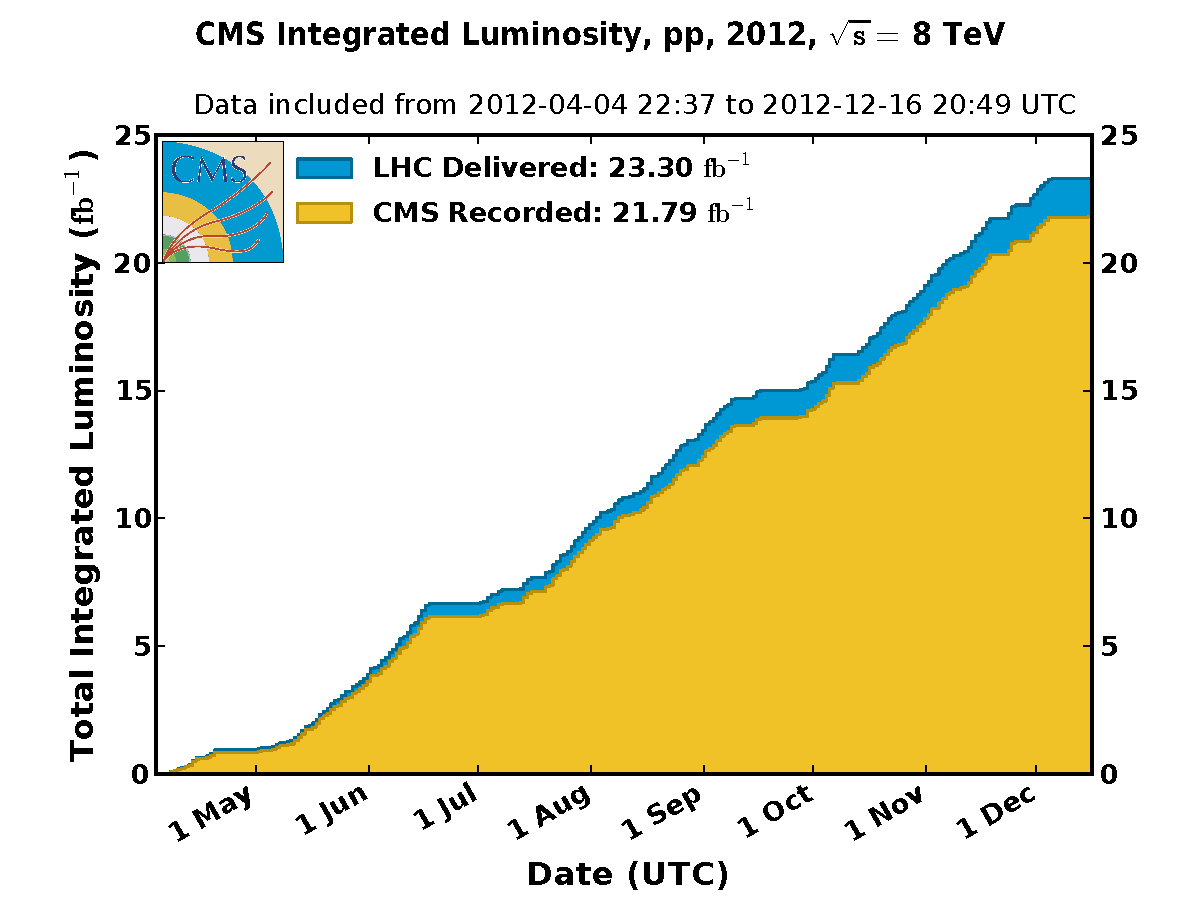
\includegraphics[width=0.49\textwidth]{figDetector/int_lumi_per_day_cumulative_pp_2012.pdf}\label{fig:LHClumi}}
    \subfloat[]{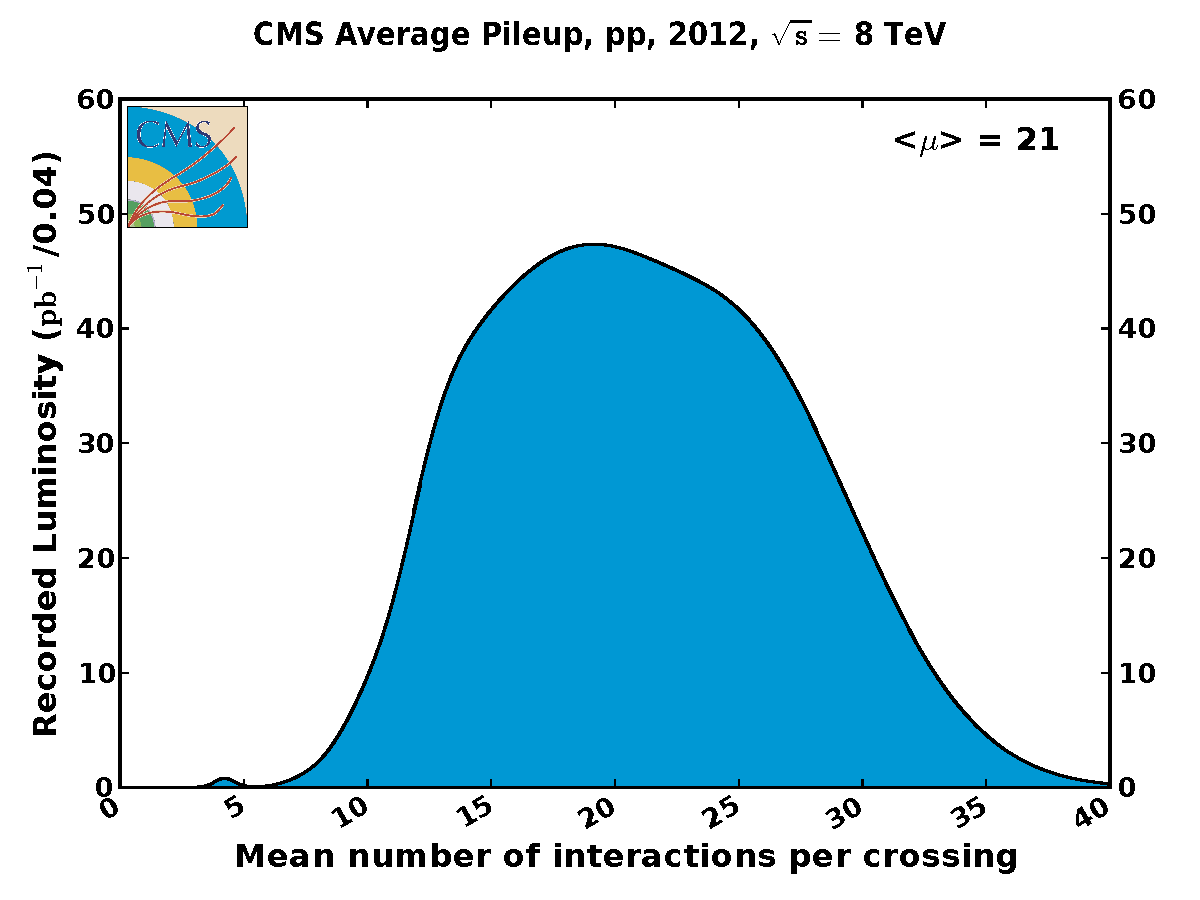
\includegraphics[width=0.49\textwidth]{figDetector/pileup_pp_2012.pdf}\label{fig:LHCpu}}
    \caption{(a) Cumulative luminosity versus week delivered to (blue), and recorded by CMS (orange) 
             during stable beams and for p-p collisions at 8~TeV centre-of-mass energy in 2012.
             (b) Mean number of interactions per bunch crossing (from Ref.~\cite{LumiPublic}).} 
    \label{fig:LHClumiPU}
  \end{center}
\end{figure}
%##########################################################################################################

LHC has already started the second period of data takingn(Run II) in April 2015, 
with a center-of-mass energy of $\sqrt{s}=13$~TeV.

%%%%%%%%%%%%%%%%%%%%%%%%%%%%%%%%%%%%%%%%%%%%%%%%%%%
\section{The CMS detector}
\label{sec:CMS}
%%%%%%%%%%%%%%%%%%%%%%%%%%%%%%%%%%%%%%%%%%%%%%%%%%%

The major characteristics of the CMS experiment~\cite{Chatrchyan:2008aa}~\cite{Bayatian:2006zz}
are summarized in its acronym. CMS is much less extendend that the ATLAS detector, 
hence it is \textbf{Compact} with a cylindrical shape of 15~\si{m}-long diameter and a length of 21.5~\si{m},
for a total weight of about 12500~\si{t}. \textbf{Muon} stands for the detector 
ability to measure very energetic muons, while \textbf{Solenoid} refers
to the shape of the magnet which the detector is built around.


\subsection{Detector requirements}
\label{subsec:CMSconcept}

CMS is installed 100~\si{m} underground at the LHC interaction point 5 (P5)
near to the Cessy village in France. As the ATLAS detector, CMS has been designed in the early 1990s 
with the aim of achieving several goals, based on a wide range of physics phenomena at the \tev scale.
The discovery of the standard model Higgs boson constituted the benchmark which the experiment 
has been built for. Additionally, the precise measurements
of additional standard model processes (QCD, electroweak, flavour physics, etc.), 
the search for supersymmetric particles and new massive vector bosons, complete
the challenge physics programme the CMS detector has been built to fulfill.
The requirements needed to achieve such a goal are:

\begin{itemize}
\item good muon identification and momentum resolution over a wide range of 
momenta with a di-muon mass resolution of $\approx$1\% at 100~\gev/\si{c}$^2$;
\item good charged particle momentum resolution and high reconstruction efficiency 
of the tracks; 
\item good electromagnetic energy resolution, with a di-photon and di-electron mass resolution 
of $\approx$1\% at 100~\gev/\si{c}$^2$ and a wide geometric coverage.
Good ability to detect the direction of the photons and the
correct position of the primary vertex, together with an efficient 
isolation of photons and leptons, crucial to reject the $\pi^{0}$ background;
\item excellent resolution measurement of the missing transverse energy (\met) 
and the di-jet invariant mass. This is possible using a hermetic hadron calorimeter 
with a broad coverage geometry.
\end{itemize}

The number of pileup events (21 on average as already seen in Figure~\ref{fig:LHCpu}) 
makes the reconstruction of each single vertex and the assignment of its respective 
tracks very challenging. Therefore, sub-detector with high granularity are required. 
The 25~\si{\ns} bunch spacing constraints the trigger system, the time-response of each sub-detector 
and the readout to cope with a collision rate of 40~\si{\mega\hertz}. Additionally, the high
radiation levels, due to copious flux of particles, requires radiation-hard detectors and front-end electronics.

\subsection{The CMS geometry}
\label{subsec:CMSgeometry}

The CMS apparatus has a cylindrical symmetry around the beam axis and it is
segmented into a central part, called \emph{barrel}, and two lateral components, called 
\emph{endcaps}. As can be observed from the schematic overall layout of the CMS detector
in Figure~\ref{fig:CMSview}, each CMS sub-detector is hosted in both the barrel and the endcap regions.

%##########################################################################################################
\begin{figure}[hbt]
  \begin{center}
    \includegraphics[width=0.98\textwidth]{figDetector/cms_complete_labelled.png}
    \caption{Tridimensional representation of the CMS apparatus (from Ref.~\cite{Chatrchyan:2008aa}).} 
    \label{fig:CMSview}
  \end{center}
\end{figure}
%##########################################################################################################

The origin of the coordinate system adopted by CMS coincides with the nominal collision point,
which is located inside the experiment. The $y$-axis points vertically upward,
the $x$-axis radially inward toward the center of the LHC, and the $z$-axis
along the beam direction toward the Jura mountains from LHC P5. 
The azimuthal angle $\phi\in[-\pi,+\pi]$ is measured from the $x$-axis 
in the transverse $x$-$y$ plane. The polar angle $\theta$ is measured with respect to the $z$-axis. 
Instead of the polar angle $\theta$, the pseudorapidity $\eta$, defined as

%##########################################################################################################
\begin{equation}
\eta=-\ln\left [\tan\left(\frac{\theta}{2}\right)\right]\mbox{ ,}
\end{equation}
%##########################################################################################################

is used as it is invariant under Lorentz boosts along the $z$ axis.

%A schematic rapresentazion of the CMS coordinate system is shown in Figure~\ref{}
%##########################################################################################################
%\begin{figure}[hbt]
%  \begin{center}
%    \includegraphics[width=0.68\textwidth]{figDetector/cms_coordinates.png}
%    \caption{Tridimensional representation of the CMS apparatus.} 
%    \label{fig:CMSview}
%  \end{center}
%\end{figure}
%##########################################################################################################


Other Lorentz invariants are the transverse momentum $p_T$ defined as
%##########################################################################################################
\begin{equation}
p_T=\sqrt{p^2_x+p^2_y}\mbox{ ,}
\end{equation}
%##########################################################################################################
where $p_x$ and $p_y$ are the projections of the particle-four momentum $p^\mu$ on the $x$ and the $y$ axes, 
respectively, the transverse energy $E_T=E\sin\theta$, and the distance $\Delta R$ between two particles with difference in 
pseudorapidity and azimuthal angle equal to $\Delta\eta$ and $\Delta\phi$, respectively:
%##########################################################################################################
\begin{equation}
\Delta R=\sqrt{ \Delta\eta^2 + \Delta\phi^2 }\mbox{ .}
\end{equation}
%##########################################################################################################

In terms of pseudorapidity, the barrel covers the range $|\eta|\le1.5$, 
while endcaps cover the range $1.5\le|\eta|\le3.0$. The presence of
additional sub-detectors until $|\eta|\le5.0$ ensures a wide coverage in acceptance.  

The description of the entire CMS apparatus is provided in the following sections.
starting from the magnet and then continuing with the sub-detectors closest to the
 interaction point up to the most external ones.
 
\subsection{Magnet}
\label{subsec:magnet}

In order to achieve a high momentum resolution in a very compact detector,
a solenoidal superconducting magnet generating a magnetic field of 3.8~\si{\tesla} is used. 
The solenoid configuration, on the contrary of a toroidal one, which is used by ATLAS,
has the advantage of producing a magnetic field that has a direction 
parallel to the beams, thus curving the muon track in transverse plane. 
The small size of the beams in this plane allows to measure the transverse 
position of the vertex with an accuracy of $\le20$\si{\mum}. 
With a solenoid magnetic field, the measurement of the track-momentum starts directly 
at the interaction point ($r=0$), while with a toroid, that starts over the absorber (typically at $r>4$~\si{\metre}.
In the first case the length of the magnetic volume is greater with respect
to the second one and this implies a better resolution. 
At the same power of curving, thus, a solenoid is more compact than a toroid.
The CMS magnet is $12.9$~\si{\metre} long and it is constituted by an internal bore
with a radius of $5.9$~\si{\metre}, which contains the tracker system and
the calorimeters. The magnet is composed of $2168$ turns and it is cooled
at the temperature of $-268.5~\si{\degreeCelsius}$. The return field is guided
by an external iron-yoke, which is $1.55$~\si{\metre} and $1.45$~\si{\metre} thick
in the barrel and in the endcap, respectively.

\subsection{Inner tracking system}
\label{subsec:tracker}

The inner tracking system is the most internal CMS sub-detector.
The main purpose of tracker is the reconstruction of 
the charged particle tracks, the primary and the secondary interaction vertices 
in the acceptance region of $|\eta|<2.5$. 
It has been designed to reconstruct tracks with a transverse momentum resolution
of $\delta p_T/p_T \approx 15\cdot p_T(GeV)\bigoplus 0.5\%$ in the central region
($|\eta|<1.6$), gradually degrading to $\delta p_T/p_T \approx 60\cdot p_T(GeV)\bigoplus 0.5\%$ 
as $|\eta|$ approaches to $2.5$. 


In order to cope with the high flux of charged primary particles coming out from each collision
($\mathcal{O}(10^3)$), whose measurement and reconstruction require high granularity and
fast time response, the CMS tracker system has been fully built in silicium.
The technology used is totally driven by the decrease of the charded-track density 
with the increase of the distance to the interaction point. Silicon pixel detectors are used 
in the region closest to the interaction point ($r<20$~\si{cm})
where a very high granularity is needed, while silicon microstrip detectors are used elsewhere.
A schematic view of the inner tracker is shown in Figure~\ref{fig:trackerLayout}.

%##########################################################################################################
\begin{figure}[hbt]
  \begin{center}
    \includegraphics[width=0.98\textwidth]{figDetector/trackerLayout.png}
    \caption{Schematic layout of CMS tracker. The main components are visible:
             Pixel Detector (PIXEL), Tracker Inner barrel (TIB), Tracker Outer barrel
             (TOB), Tracker Inner Disk (TID), Tracker endcap (TEC) (from Ref.~\cite{Chatrchyan:1704291}).} 
    \label{fig:trackerLayout}
  \end{center}
\end{figure}
%##########################################################################################################

The pixel detector consists of matrices of $100\times150$~\si{\mum} silicon pixels
arranged on three concentric barrel layers and four endcap disks, two per
each extremity, as can be seen from the Figure~\ref{fig:pixelLayout}. 
The barrel layers are positioned at distance $r=4.4$, $7.3$ and $10.2$~\si{cm} 
from the beam line, while the endcap disks are located at $|z|=34.5$ and $46.5$~\si{cm}.
As shown in Figure~\ref{fig:pixelBarrel}, in the barrel there is an overlap of 6\%
in $\phi$ in order to benefit from the effect of the Lorentz force on the spatial resolution.
Thanks to the large deflection Lorentz-angle created by the magnetic field
on the trajectory of the charged particles is possible to obtain a resolution of $10$~\si{\mum} 
along $\phi$ and $\approx 20$~\si{\mum} along $z$. Also in the endcap disks, the sensors 
are arranged in a ``turbine'' geometry (the blades are rotated by $20~\si{\degreeCelsius}$) 
in order to benefit from the Lorentz effect. The total active area of the pixel detector is of about 1~\si{m}$^2$.

%##########################################################################################################
\begin{figure}[h!]
  \begin{center}
    \subfloat[]{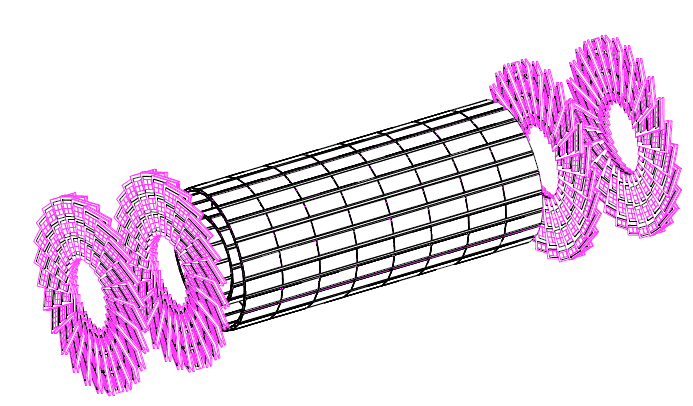
\includegraphics[width=0.74\textwidth]{figDetector/pixelLayout.png}\label{fig:pixelLayout}}
    \subfloat[]{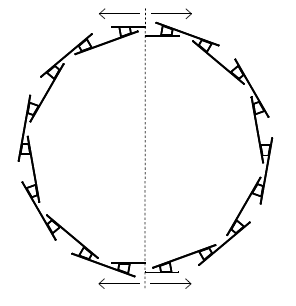
\includegraphics[width=0.24\textwidth]{figDetector/pixelBarrel.png}\label{fig:pixelBarrel}}
    \caption{(a) Perspective view of the CMS pixel system. (b) Radial cut of the mechanical 
	    frame of first layer of the barrel (from Ref.~\cite{Karimaki:368412}).} 
    \label{fig:pixels}
  \end{center}
\end{figure}
%##########################################################################################################

As already anticipated with the Figure~\ref{fig:trackerLayout}, the most external layers of 
the tracker are further, for which the micro-strip technology has been used, is further divided into: 
Tracker Inner and Outer Barrel (TIB and TOB, respectively), Tracker Inner Disks (TID) and Tracker Endcaps (TEC).
The Tracker Inner Barrel and Disks (TIB/TID) extend towards $r=55~\si{\cm}$ and are composed by 4 barrel
layers and 3 disks at each end, respectively. TIB/TID silicon micro-strip sensors have a thickness
of $320~\si{\mum}$ and a strip pitch that varies from $80~\si{\mum}$ in the innermost barrel layer 
$140~\si{\mum}$ in the outermost disks. The sensors are arranged parallely to the beam axis
in the barrel and radially in the disks, providing four $r-\phi$ measurement on the charged track.
The TIB/TID system is surrounded by the TOB, which is extended up to $r=116~\si{\cm}$. It is
composed by 6 layers of $500~\si{\mum}$ thick micro-strip sensors with a strip pitch 
of $183~\si{\mum}$ for the first four layers and $122~\si{\mum}$ for the last two ones.
The TOB provides 6 additional measurements.
% with a resolution of $53~\si{\mum}$ in $r-\phi$ and $35~\si{\mum}$ in $z$. 
In the endcaps, the TEC extends in the region $124~\si{\cm}<|z|<282~\si{\cm}$ 
and $22.5~\si{\cm} < |z|< 113.5~\si{\cm}$. The TEC is composed by 9 disks, providing up to 9 $\phi$
measurements per trajectory. Each disk is constituted by 7 rings of silicon micro-strip detectors 
with a thickness varying from $320~\si{\mum}$ for the first 4 rings, to $500~\si{\mum}$
for the last two rings and with an average pitch varying from $97~\si{\mum}$ to $184~\si{\mum}$
depending on the distance from the beam line. 

The first two layers and rings, respectively, of TIB, TID, and
TOB as well as rings 1, 2, and 5 of the TEC are made with ``stereo'' modules in 
order to provide a measurement in both $r-\phi$ and $r-z$ coordinates. These components
have a second micro-strip detector module which is mounted back-to-back with an angle of $100~\si{\milli\radian}$.

\subsection{Electromagnetic Calorimeter}
\label{subsec:ecalo}

The CMS Electromagnetic Calorimeter (ECAL)~\cite{ecalTDR} has the main function of measuring
the energy of particles that generate electromagnetic showers (i.e. photons and electrons).
It is placed outside the tracker, inside the coil of the magnet. 

The ECAL is an homogeneous calorimeter whose active material is a crystal scintillator 
made of lead tungstate (PbWO$_4$). The calorimeter is divided into two parts: 
the ECAL Barrel (EB), which covers the pseudorapidity range $|\eta|< 1.479$
and consists of $61200$ crystals, and ECAL Endcaps (EE), which cover the range $1.479<|\eta|<3$ and consist of $7324$ crystals each.
The most distinguising feature of the CMS ECAL is the lead tungstate scintillating crystals, which
have a short radiation lenght ($X_0=0.89~\si{\cm}$, being $X_0$ the distance needed to attenuate incident 
radiation of a factor $1/e$) and a small Moli\`ere radius ($R_M=2.2~\si{\cm}$). These
features garantee an excellent containment of the showers in a compact volume with high granularity.
Indeed, crystal-lenghts of $23~\si{\cm}$ in the barrel and $22~\si{\cm}$ in the endcaps are enough
to collect almost all the average particle energy. Both barrel and endcap crystals are
displaced off-point from the nominal vertex position to mitigate the detection inefficiency
on the surface, but while barrel crystals are arranged in an $\eta-\phi$ grid, endcap crystals are arranged in an $x-y$ one.

Together with tightness, compactness and high granulairty, the crystals used have a very fast response
given that the 80\% of the scintillation light is emitted in $25~\si{\ns}$. The crystals are also radiation resistant. 
One of the defects of this kind of crystal is that a large amount
of the stored energy is dissipated through thermal emission, then, in order to cope with the relatively low light yield 
($30\gamma$/\si{\MeV}), photodetectors with intrinsic gain and able to operate in a high magnetic field are used.
Silicon avalanche photodiodes (APDs) are used as photodetectors in the barrel and
vacuum phototriodes (VPTs) in the endcaps. Moreover, given that the sensitivity of both the crystals
and the APD changes with the temperature, the thermal regulation is needed and carried out by a cooling circuit which 
keeps the operating temperature at ($18\pm0.05$)~\si{\degreeCelsius}. 

A preshower device (ES) is placed in front of the EE, covering the pseudorapidity range 
$1.653<|\eta|<2.6$. It is a sampling calorimeter composed by two layers of
lead radiator, behind each of that silicon strip sensors are placed.
The preshower is mostly designed to discriminate genuine photons from those
coming from the electromagnetic decay of a neutral pion, but it also leads to an improvement in the 
electrons identification and in the accuracy in determining electrons and photons position.
The longitudinal view of one quarter of the CMS ECAL is shown in Figure~\ref{fig:ecalLayout}.

%##########################################################################################################
\begin{figure}[hbt]
  \begin{center}
    \includegraphics[width=0.98\textwidth]{figDetector/ecalLayout.png}
    \caption{Longitudinal view of one quarter of the CMS ECAL detector in which the ECAL Barrel (EB), the ECAL Endcap (EE) and the Preshower
             (ES) are visible.  
             The dashed lines correspond to fixed $\eta$ values (from Ref.~\cite{Chatrchyan:2008aa}).} 
    \label{fig:ecalLayout}
  \end{center}
\end{figure}
%##########################################################################################################

The ECAL energy resolution, measured using electron beams with energy
between $20$ and $250~\si{\GeV}$, can be parametrized as: 
%##########################################################################################################
\begin{equation}
    \left(\frac{\sigma}{E}\right)^2= \left(\frac{a}{\sqrt{E}}\right)^2 + \left(\frac{\sigma_N}{E}\right)^2 + c^2\mbox{      (with E in \si{\GeV}).}
    \label{eq:resolutionECAL}
\end{equation} 
%##########################################################################################################
The stochastic term $S$ includes the statistical behavior of the interaction
processes, such as fluctuations on the energy containment and photo-statistics. The term $N$ takes into account
the noise associated to the electronics and the pileup, and the constant term $C$
is related to the calorimeter features (i.e. inter-calibration errors, geometrical effects, etc.). 
The energy resolution test-beam results are summarized in Table~\ref{tab:ecalRes}.

\begin{table}[htp]
\begin{center}
\caption{ECAL energy resolution contributions in barrel and endcap. The unit of measurement for
the energy $E$ is \si{\GeV}~\cite{ecalTDR}.}
\label{tab:ecalRes}
\begin{tabular}{cc|c|c|}\\
\cline{2-4}
                               & \multicolumn{1}{|c|}{$a$}               & $\sigma_N$              & c \\\hline
\multicolumn{1}{|c|}{Barrel}   & $2.7/\sqrt{E}$    & $0.155~\si{\GeV}$       & $0.55\%$\\
\multicolumn{1}{|c|}{Endcap}   & $5.7/\sqrt{E}$    & $0.205~\si{\GeV}$       & $0.55\%$\\
\hline
\end{tabular}
\end{center}
\end{table}


\subsection{Hadronic Calorimeter}
\label{subsec:hcalo}

The Hadron Calorimeter (HCAL)~\cite{hcalTDR} has the main function of measuring the charged and neutral 
hadron energy and also providing a more hermeticity for the measurement of \met.
It is divided into the HCAL Barrel (HB), which covers the pseudorapidity range $|\eta|<1.4$ and the
HCAL Endcap (HE), which is extended in the range $|\eta|<1.4$ and $1.3<|\eta|<3.0$,
as can be seen from Figure~\ref{fig:hcalLayout}.

%##########################################################################################################
\begin{figure}[hbt]
  \begin{center}
    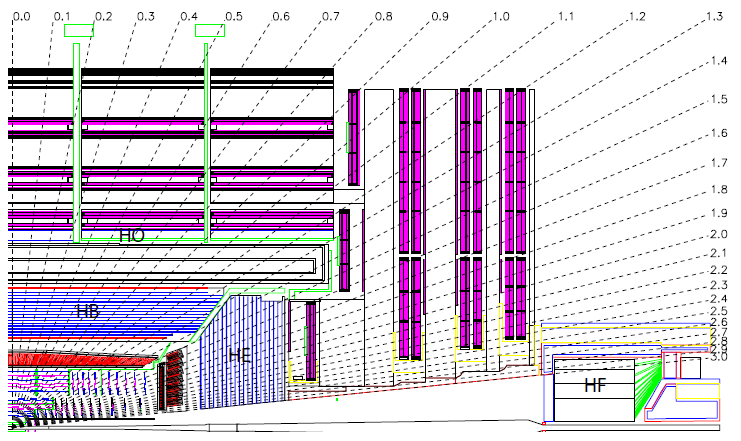
\includegraphics[width=0.98\textwidth]{figDetector/HCALlayout.png}
    \caption{Longitudinal view of the CMS detector in which the different components of the HCAL are visible:
             the Hadron Barrel (HB), Endcap (HE), Outer (HO) and Forward (HF) calorimeters. 
             The dashed lines correspond to fixed $\eta$ values (from Ref.~\cite{Chatrchyan:2008aa}).} 
    \label{fig:hcalLayout}
  \end{center}
\end{figure}
%##########################################################################################################

HCAL is a sampling calorimeter, meaning that differently from the fully active ECAL,
it is constituted by layers of a dense absorber alternated with an active medium.
Both HB and HE are placed on the outer side of the ECAL and inside the coil of the solenoid. 
%because of the greater longitudinal extension of the hadronic showers 
%with respect to the electromagnetic ones, and inside the coil of the solenoid.  
Given that both HB and HE are placed on the outer side of the ECAL and inside the coil of the solenoid,
the vicinity to the intense magnetic field requires the usage of non-ferromagnetic materials.
Stainless steel and copper alloys (brass) have been chosen as absorbers, while tiles 
of plastic scintillator as active medium. Each scintillator is read out with embedded wavelength-shifting (WLS) fibers, connected to 
high-attenuation-length clear fibers, which convey the light signal to the readout system,
where is amplified by hybrid photodiode (HPD).

The high granulatiry in $\eta-\phi$ is obtained by segmenting the scintillators 
from $\Delta\eta\times\Delta\phi=0.087\times5$~\si{\degreeCelsius} in the barrel up to 
$\Delta\eta\times\Delta\phi=0.35\times10$~\si{\degreeCelsius} in the endcaps.
The HCAL thickness, in terms of nuclear absorption length $\lambda_I$, goes from approximately 
$5.82~\lambda_I$ in the barrel up to $10.6~\lambda_I$ in the endcaps. However, the barrel-depth is not enough to 
contain the full shower, then an additional module, the HCAL Outer (HO), is placed
outside the magnet. The HO detector, which covers the region $|\eta|<1.26$ (Figure~\ref{fig:hcalLayout}), 
contains scintillators serving as ``tail-catcher'', given that they sample the energy from penetrating hadron showers 
leaking through the rear of the calorimeters. The forward HCAL (HF) extends the acceptance of the 
detector to the region $3.0<|\eta|<5.2$ and it is located $11~\si{\m}$ away from the interaction point 
(Figure~\ref{fig:hcalLayout}). This location makes the HF working in an high-radiation dose environment, 
for this reason the material chosen as absorber is steel embedded with quartz fibers, used as active material. 
The fibers, once crossed by the the hadornic shower, produce light due to Cherenkov effect.
The inclusion of the HO layers extends the total depth of the calorimeter system to a minimum of $11~\lambda_I$.

The energy resolution is $\sigma/E=65\%/\sqrt{E}\oplus5\%$ in the barrel, $\sigma/E=83\%/\sqrt{E}\oplus5\%$
in the endcaps and $\sigma/E=100\%/\sqrt{E}\oplus5\%$ in the HF~\cite{hcalTDR}.

\subsection{Muon system}
\label{subsec:muonsys}

Muons play a major role in the most of the appealing SM and exotic scenarii made available by the 
LHC physics programme. Muon detection was crucial for the discovery of the SM Higgs boson in the golden-channel
H$\rightarrow$ZZ$^*$, decaying in four leptons, or also for the observation of the rare decay 
B$^0_S\rightarrow\mu^+\mu^-$~\cite{CMS:2014xfa}.
For these reasons, a sophisticated and complex system has been built to reconstruct muons and 
measure their kinematics properties, but also to fulfill the function of event-trigger.
Given the need to cover a large area affected by a magnetic field of variable intensity and 
radiation, three different kind of gas-ionization detectors have been used in the muon system~\cite{CMS:1997dma},
as can be seen from the Figure~\ref{fig:muLayout}: the Drift Tubes (DT), the Catode Strip Chambers (CSC), 
and the Resistive Plate Chambers (RPC).

%##########################################################################################################
\begin{figure}[hbt]
  \begin{center}
    \includegraphics[width=0.98\textwidth]{figDetector/muonLayout.png}
    \caption{Longitudinal view of the CMS detector in which the different components of the muon system are visible:
             the Drift Tubes (DT), the Catode Strip Chambers (CSC), and the Resistive Plate Chambers (RPC).
             The dashed lines correspond to fixed $\eta$ values (from Ref. ~\cite{Chatrchyan:2013sba}).} 
    \label{fig:muLayout}
  \end{center}
\end{figure}
%##########################################################################################################

The DT chambers are made up a $50~\si{\mm}$-thick gold-plated stainless-steel anode wire and an aluminum strip cathode, 
placed on the shortest side of the cell. The cell is filled with a gas mixture of CO$_2$ (85\%) and Ar (15\%). 
Because of their time-response ($\approx400~\si{\ns}$~\cite{Chatrchyan:2013sba}), the DT suit as tracking detectors 
in the barrel region ($|\eta|<1.2$), where the muon flux is weak ($<10~\si{\hertz}/\si{\cm}^2$) and the residual magnetic field is low.  
The barrel region is segmented in five wheels, $2.5~\si{\m}$ long. Each wheel is divided into 12 sectors and 
one single sector consists of $250$ drift tubes chambers arranged in four stations (MB1, MB2, MB3, MB4, with MB standing for
Muon Barrel), each interspersed by an iron-yoke layer. Chambers are staggered to avoid gaps between each other (\emph{crack}) and, thus, muons leaving unmeasured 
the detector. The MB4 station provides the $\phi$ coordinate measurement only, while MB1, MB2 and MB3, consisting of twelve 
planes of drift tubes, lead to eight measurements in the $r-\phi$ projection and four along the $z$-axis.
Then, given the higher number of hits available, the radial resolution ($100~\si{\mum}$) is better than the one
associated to the $z$-direction ($150~\si{\mum}$). The angular resolution in $\phi$ is $1~\si{\mrad}$.

The CSC detector is placed in the endcap regions ($0.9<|\eta|<2.4$), characterized by a high radiation dose
and a large, non-uniform magnetic field. The Muon Endcap (ME) system consists of four stations of CSC (ME1, ME2, ME3, ME4), each
interleaved by one layer of the magnet iron-yoke. Each chamber has a trapezoidal shape and is filled with 
a gas mixture of Ar (40\%), CO$_2$ (50\%) and CF$_4$ (10\%). Additionally, it consists of six gaps, each
made of a multi-wire anode layer interspersed by a cathod-strips planes. Wires are $\phi$-oriented and 
perpendicularly arranged with respect to the strips, which are segmented radially. 
In each gap, six space measurements are provided: $\phi$ is measured by calculating the center of gravity 
of the ionic charge induced by avanlanche on the strips once the gas has been inozide, while 
$r$ is obtained by the electronic charge collected on the anode. The single point resolution 
is of about $75$-$150~\si{\mum}$ in $\phi$ and $200~\si{\mum}$ in $r$.

As can be seen from the Figure~\ref{fig:muLayout}, a set of RPC is placed both in the barrel ($0<|\eta|<1.2$), 
and in the endcaps ($0.9<|\eta|<1.6$). The double-gap RPC detectors consist of two single-gap chambers operating in avalanche mode. 
Both units are assembled back-to-back in order to share a segmented pick-up read-out strips 
in between, which allows the usage of a lower high voltages (HV) in each single-gap with an effective gain in efficiency. 
Each chamber consists of two bakelite-electrodes externally covered by a layer of graphite, which is used
as HV electrode. The whole unit is covered by mylar sheets, serving as HV insulators.
The gap between the electrodes is $2~\si{\mm}$-thick and is filled with a gas mixture of C$_2$H$_2$F$_4$ (96\%), 
C$_4$H$_{10}$ (3.5\%) and SF$_4$ (0.5\%). Not ideal for space measurement given the coarse spacial resolution, 
the RPCs are, instead, crucial for the even-triggering, having a high rate responses (up to $10~\si{\kilo\hertz}/\si{\cm}^2$).


\subsection{Trigger and Data acquisition}
\label{subsec:triDAQ}

At the design luminosity ($\mathcal{L}=$10$^{34}$\cm$^{-2}$\si{s}$^{-1}$), the LHC protons crossing frequency 
($40~\si{\mega\hertz}$ for $25~\si{\ns}$ spaced beams) translates into $\approx 20$ inelastic interactions per bunch crossing and 
$\approx 1~\si{\mega\byte}/$event of zero-suppressed data in the CMS read-out systems. Performing a permanent storage of such 
amount of data is technically awkward, therefore a drastic rate reduction must be achieved. To accomplish this goal, a trigger and 
data acquisition (TriDAQ) system is used. CMS adopts a two-level system of rate reduction, which consists of a 
Level-1 (L1) Trigger~\cite{Bayatyan:706847}, followed by a High-Level Trigger (HLT)~\cite{Sphicas:2002gg}.

The L1 trigger is a real on-line and hardware-based event filter. It reduces the data-rate of a factor $\mathcal{O}(10^3)$,
providing an output rate limit of $100~\si{\kilo\hertz}$. During the finite L1 trigger latency-time of $3.2~\si{\mum}$, 
in which the trigger decides whether accepting an event or not, 128 bunch-crossing information are stored in pipelined FIFO memories.
Due to the short decision-time, only the information provided by the calorimeters and the muon system are exploited.
In particular, for trigger purposes, calorimeters are segmented into \emph{trigger towers} with a size equal to
$0.087\times 5^\circ$ in $\Delta\eta\times\Delta\phi$ up to $|\eta|<1.74$ and larger at higher $\eta$ values.
ECAL, HCAL, HF, DTs, CSCs and RPCs contribute to build the L1 trigger components at different levels: \emph{local}, \emph{regional} and 
\emph{global}. The local components are extracted from energy deposits measured in the calorimeter trigger towers, 
and track segments or hit patterns in the muon chambers. These primitives are then combined to build
trigger objects which give rise to the regional components. At this level, DTs and CSCs join segments to complete 
the muon tracks, while the RPCs perform unambiguously the tracks/bunch-crossing matching. In the calorimeters, the electron
and photon identification is performed and additional information about muon isolation and compatibility with 
minimally ionizing particles (MIP) are also collected. Once measured, all these regional components are ranked according to 
whether they meet or not some thresholds and quality requirements. The highest-ranked components are then built indipendently by 
the Global Calorimeter Trigger (GCT) and the Global Muon Trigger (GMT) and transferred to the final Global Trigger (GT), 
the top entity of the Level-1 hierarchy. At this point, based on the best muon, electron and photon candidates found, 
and the measured $E_T$, \met, number of jets, and scalar sum of some hadronic activity ($H_T$), 
the L1 trigger decides whether rejecting the event or not. 

Once the L1 trigger processing is finished, data are read-out from the detector through the 
Data Acquisition System (DAQ). Thus the complete information is passed to the event builder network, and then to 
the fully-software based HLT system. The HLT reduces the data-rate to about $100~\si{\hertz}$ in about $10~\si{\mum\s}$
for most of the event processed. The main pillar which the HLT algorithms are based on is the ~\emph{regional reconstruction}:
the idea is processing only those events found already interesting by the L1 trigger and fastly discard all the rest in 
order to maximize the latency reduction. This has led to the development of three ``virtual'' trigger levels: the first level 
accesses only the muon and calorimetric data, the second level includes the information provided by the tracking system.

Given the strong algorithm flexibility, the HLT ``menu'' has been enriched, in the last few years, 
with many HLT sets of \emph{trigger paths}, each customized to be tuned with the collider configuration.

\subsection{CMS software, computing and simulation}
\label{subsec:CMSsim}

Events accepted by the HLT are finally written on disks and made available for offline-data analysis by an off-line system of computing~\cite{CMS:2005aa}.
The world-wide scale of data distribution has given rise to the need of having a common software framework,
%\footnote{The CMS software framework is called \texttt{CMSSW} and it is a collection of tools and algorithms used for the event simulation and reconstruction.}
and a common infrastructure of data-storage. The former, an object-oriented framework written in \texttt{C++} and \texttt{Python},
is fully customizable for any computer architecture and it is constantly developed in a high-performance, flexible and manageable way. 
The latter has the name of Worldwide LHC Computing Grid (WLCG) and it is used by physicist all around the world to access CMS data. 
It consists of a computing and storage system distributed among different terminals around the world, each of which is interfaced with a backup-base at CERN: the Tier0 (T0).
The T0 receives data from the CMS TriDAQ system and organizes them in Primary Dataset (PD) depending on the associated HLT paths. 
Examples of PD are provided by those will be used in the analyses described in this thesis: \texttt{DoubleMuon} and \texttt{DoubleElectron}.
The datasets are then sent to Tier1 (T1) centers, which are systems of permanent storage, but which also provide the necessary CPU for
skimming and calibration processes. More numerous and smaller are the Tier2 (T2) centers, characterized by conspicuous CPU resources able
to provide capacity for analysis, calibration activities and Monte Carlo (MC) simulation. 

On the way of deeply understanding the detector effect in order to properly optimize the analysis strategies,
MC processes play a crucial role. The simulation workflow starts with the usage of MC generators to 
generate the interesting process, after having fixed the theoretical model behind. Several MC generators are available
to suit a wide range of physics processes and few of them will be described in details in the Section~X.Y. 
Once generated, the propagation of the particles inside the detector, and the interaction with its components, 
is simulated using the Geant4 toolkit~\cite{Agostinelli:2002hh}. Geant4 also models the geometry of the different CMS subdetectors, 
the map of the magnetic field and the front-end electronic. At the end of the chain, the whole trigger system is modelled and the simulated event
is ready to be written on disks and be fully reconstructed as if it was a real data event.





























